\documentclass[a4paper,14pt]{extarticle}
% extbook, extarticle --- для больших шрифтов.
\usepackage[left=23mm,right=13mm,top=20mm,bottom=20mm]{geometry}
% геометрия страницы
% landscape --- альбомная ориентация

% 1em --- ширина глифа m в выбранном текущем шрифте
% 1ex --- ширина и высота глифа x

% гуглить package_name.sty

% \parindent=1cm % абзацный отступ

% локализация:
\usepackage[T2A]{fontenc} % шрифтовая кодировка
% T2A --- для кириллических файлов
\usepackage[utf8]{inputenc} % кодировка исходного файла
% utf8 --- база, cp1251 --- ????, cp866 --- для дедов (DOSовская), koi8r --- экзотика
\usepackage[english, russian]{babel} % (вавилон) --- загрузка национальной инфографики
% несколько языков --- последняя по умолчанию
% переключение --- \selectlanguage{language}
\usepackage{indentfirst} % красная строка после заголовков
\usepackage{amsmath, amsfonts, amssymb} % база от AMS

\usepackage{graphicx} % картинки
\graphicspath{{./images/}}

\usepackage{xcolor} % красить текст

%\pagecolor[rgb]{0.01,0.01,0.01}
%\color[rgb]{0.95,0.93,0.80}
%тёмная тема

\usepackage{faktor} % красивое фактор-множество

\usepackage{ragged2e} % центрирование и иже с ним

\usepackage{multicol} % слияние колонок и строк таблиц

\usepackage{array} %приколы со средой array

\usepackage{enumitem}
% для тонкой настройки параметров списков
\setlist[itemize,enumerate]{before={\vspace{-2\parsep}},after={\vspace{-1.5\parsep}},itemsep=-1\parsep}
\setlist[enumerate,2]{before={\vspace{-2\parsep}},after={\vspace{-2\parsep}},itemsep=-0.75\parsep}

\allowdisplaybreaks

\DeclareMathOperator{\Ln}{Ln}
\DeclareMathOperator{\Ree}{Re}
\DeclareMathOperator{\Imm}{Im}
\DeclareMathOperator{\CC}{\mathbb{C}}
\DeclareMathOperator{\RR}{\mathbb{R}}
\DeclareMathOperator*{\res}{res}
\DeclareMathOperator*{\normallimsup}{\overline{lim}}

\DeclareMathOperator{\NN}{\mathbb{N}}
\DeclareMathOperator{\QQ}{\mathbb{Q}}

\DeclareMathOperator{\Cov}{Cov}

% равномерная сходимость.....
\makeatletter
\newcommand*{\relrelbarsep}{.386ex}
\newcommand*{\relrelbar}{%
    \mathrel{%
        \mathpalette
        \@relrelbar
        \relrelbarsep
    }%
}
\newcommand*{\@relrelbar}[2]{%
    \raise#2\hbox to 0pt
        {$\m@th#1\relbar$\hss}%
    \lower#2\hbox{$\m@th#1\relbar$}%
}
\providecommand*{\rightrightarrowsfill@}{%
    \arrowfill@\relrelbar\relrelbar\rightrightarrows
}
\providecommand*{\xrightrightarrows}[2][]{
    \ext@arrow 0359\rightrightarrowsfill@{#1}{#2}
}
\makeatother

\newcommand{\norm}[1]{\left\Vert #1 \right\Vert}
\newcommand{\abs}[1]{\left\vert #1 \right\vert}
\newcommand{\scmult}[1]{\left\langle #1 \right\rangle}
\DeclareMathOperator{\sgn}{sgn}
% равномерная сходимость.....

\makeatletter
\renewcommand*\env@matrix[1][*\c@MaxMatrixCols c]{
    \hskip -\arraycolsep
    \let\@ifnextchar\new@ifnextchar
    \array{#1}
}
\makeatother
% добавляем возможность форматировать матрицы как таблицы, например рисовать вертикальную черту перед столбцом свободных членов при решении неоднородных уравнений

\usepackage{tikz}
\newcommand*\circled[1]{\tikz[baseline=(char.base)]{
    \node[shape=circle,draw,inner sep=1pt] (char) {#1};}}
%обводим равно (или вообще что захочется) в кружочек

\usepackage{amsthm} % теоремки теоремочки
\newtheorem{theo}{Теорема}[section]
\newtheorem{examp}{Пример}[section]
\newtheorem{cor}{Следствие}[theo]
{
    \theoremstyle{remark}
    \newtheorem{remark}{Замечание}[section]
    \newtheorem{exerc}{Упражнение}
}
{
    \theoremstyle{definition}
    \newtheorem*{prf}{Доказательство}
    \newtheorem{defin}{Определение}[section]
}

\usepackage{cancel} %КАНСЕЛ

\usepackage{pdfpages} %вставка титульника

\usepackage[labelsep=period]{caption} %подписи к рисункам с разделителем точкой

\usepackage[shortcuts]{extdash} %перенос составных слов, содержащих тире

\begin{document}

    \includepdf{tit.pdf}

    \tableofcontents

    \newpage

    \section*{Введение}
    \addcontentsline{toc}{section}{Введение}

    Магнитные анизотропные частицы в последние несколько лет стали независимой быстроразвивающейся отраслью в исследованиях мягких материалов~\cite{bib:three, bib:four, bib:five, bib:six}. В конце 20-го века, системы дипольных частиц с анизотропией привлекли большое внимание со стороны ученых благодаря способности образовывать различные жидкокристаллические фазы, такие как нематическая, смектическая и другие~\cite{bib:seven, bib:eight, bib:nine, bib:ten}. Центральное место в этих исследованиях было занято системами жестких/мягких эллипсоидов или сфероциллиндров с точечным дипольным моментом, сонаправленным с главной осью (осью вращения), при этом системы с моментами более высокого порядка также были исследованы~\cite{bib:one}.

    В теории ранее были изучены основные состояния магнитных стержней и эллипсоидов с точечными диполями. Были рассмотрены две различные ориентации диполей: дипольный момент, ориентированный вдоль короткой оси анизотропной частицы и дипольный момент, расположенный вдоль длинной оси.

    Если эллипсоиды или стержни с дипольным моментом, расположенным вдоль длинной оси, достаточно вытянутые, конфигурация моментов голова-хвост становится менее подходящей, чем у пары диполей, расположенных бок о бок относительно друг друга. Этот структурный переход в основных состояниях ведет к критическим изменениям в микроструктуре систем анизотропных частиц, когда тепловая энергия начинает быть сравнимой с взаимодействием между частицами.

    Частицы с дипольным моментом, ориентированные перпендикулярно оси вращения, не были столь активно рассмотрены, и основной целью таких исследований было понять, какие новые кристаллические фазы можно приобрести путем вращения диполя. Кроме того, были изучены некоторые более сложные варианты расположения диполей. Было установлено, что система жестких эллипсоидов или сфероциллиндров с дипольным моментом, сонаправленным с главной осью, может пройти фазовый переход из
    газа в жидкость, в отличие от дипольных систем твердых сфер, где этот
    переход еще никогда не был доказан. Лишь немногие исследования были проведены для выяснения изотропной газовой фазы анизотропных дипольных частиц.


    Основные выводы из последних исследований для изотропной фазы
    заключаются в том, что для относительного высокого удлинения частицы, ориентация диполей в соседних частицах, расположенных бок о бок друг к другу, становится энергетически более выгодной, чем соотношение голова-хвост, присущее дипольным взаимодействиям сферических частиц. И скорее всего, последняя особенность парной корреляционной функции для сильно вытянутых частиц играет решающую роль в фазовом переходе и влияет на термодинамические свойства этих систем, особенно при плотностях, близких к критическим. Тем не менее, зависимость термодинамических и структурных свойств удлинения частиц при низких плотностях
    не была тщательно изучена~\cite{bib:two}.


    Недавнее <<возрождение>> магнитных анизотропных частиц было вызвано экспериментальными исследованиями, направленными на применение в медицине и микрожидкостях. Кроме того, недавно были проведены многочисленные и разносторонние эксперименты с эллипсоидами, магнитные моменты которых ориентированы вдоль короткой оси. Во всех этих экспериментах были проанализированы системы при малых концентрациях, соответствующих изотропной фазе. Межчастичные взаимодействия в некоторых из этих экспериментов являются очень сильными и приводят к агрегации.

    Все это приводит к желанию тщательно проанализировать влияние формы анизотропии частиц на их свойства и изотропные фазы и основные состояния таких систем, чтобы быть в состоянии предсказать возможные структурные переходы и кластерные топологии. В результате появилось несколько компьютерных экспериментов, показывающих особенности системы магнитных стержней в присутствии внешнего магнитного поля, но нет систематического кластерного анализа при нулевых полях, как и до сих пор не была представлена зависимость поведения от отношения полуосей
    для дипольных стержней или эллипсоидов.

    Стоит отметить, что ориентация дипольного момента относительно осей эллипсоида обязательно повлияет на микро-, и, как следствие, макросвойства системы. Так, например, более 30 лет назад, когда были сделаны первые опыты двупреломления в феррожидкостях, одним из возможных объяснений было то, что при незначительной эллипсоидальной форме, присущей кристаллической решетке феррочастиц, дипольный момент был сонаправлен с осью вращения, в отличие от эллипсоидов с кремниевой оболочкой.

    \newpage

    \section{Постановка задачи}

    Задачей данного исследования было изучить потенциалы взаимодействия в системах магнитных эллипсоидов и создать аппроксимацию для стерического потенциала Гей-Берне при произвольном заданном соотношении полуосей частицы. Упрощенный потенциал будет использован для теоретического расчета различных макроскопических параметров системы.

    Далее подробно рассмотрена постановка всей задачи.

    \subsection{Описание системы частиц}

    Магнитная часть взаимодействия характеризуется магнитным диполь\-/дипольным взаимодействием, когда диполь $m_i$ всегда находится в центре масс $i$-ой частицы, а форма отличается от сферической.

    В данной работе рассматривается случай, когда частицы представляют из себя эллипсоиды вращения с точечным магнитным моментом, расположенным, как описано выше, в центре масс частицы и направленным вдоль длинной полуоси эллипсоида.

    Соотношение сторон есть параметр $X_0 = \frac{b}{a}$, определяющий форму частицы. Мы будем рассматривать вытянутые эллипсоиды, то есть случай, когда $X_0 > 1$.

    \subsection{Потенциал Гей-Берне}

    Для описания стерического взаимодействия анизотропных частиц существует потенциал Гей-Берне. Это потенциал, который широко используется для описания частиц, находящихся на небольшом расстоянии друг от друга. При этом, потенциал Гей-Берне учитывает не только расстояние между центрами частиц, но и их ориентацию. Его выражение имеет вид:
    \begin{gather*}
        U_{GB} (u_i, u_j, r_{ij}) =
        \begin{cases}
            4 \varepsilon(u_i, u_j)
            [A^{12}(u_i, u_j, r_{ij}) - A^6(u_i, u_j, r_{ij})]
            + \varepsilon(u_i, u_j)
            & r_{ij} \leqslant r_c \\
            0, & r_{ij} > r_c
        \end{cases} \\
        A(u_i, u_j, r_{ij})
        = \frac{\sigma_0}{r_{ij} - \sigma(u_i, u_j, r_{ij}) + \sigma_0} \\
        \sigma(u_i, u_j, r_{ij})
        = \sigma_0 \left[
        1 - \frac{\chi(X_0)}{2}
        \times \frac{(\hat{r_{ij}}\cdot u_i
        + \hat{r}_{ij}\cdot u_j)^2}{1 + \chi(X_0) u_i \cdot u_j}
        + \frac{(\hat{r_{ij}}\cdot u_i
        - \hat{r}_{ij}\cdot u_j)^2}{1 - \chi(X_0) u_i \cdot u_j}
        \right]^{-\frac12} \\
        \varepsilon(u_i, u_j)
        = \varepsilon_0 \cdot [1 - \chi^2(X_0) (u_i \cdot u_j)^2]^{-\frac12} \\
        \chi(X_0) =
        \frac{X_0^2-1}{X_0^2+1} \\
        r_c = (2^{\frac16} - 1) \sigma_0 + \sigma(u_i, u_j, r_{ij}) \\
        \hat{r}_{ij} = \frac{r_{ij}}{\abs{r_{ij}}} \\
        \sigma_0 = \sqrt{2} d
    \end{gather*}

    Здесь $r_{ij}$ ($\hat{r}_{ij}$) --- (нормированный) радиус-вектор, соединяющий центры частиц, $u_i$ --- единичный вектор, направленный вдоль главной  оси частицы, $d$ --- диаметр частицы, $X_0$ --- соотношение полуосей.

    Если перейти к сферической системе координат с началом координат в центре масс первой частицы и осью $z$, сонаправленной с её магнитным моментом, то потенциал выразится через расстояние $r$ и углы между частицами $\theta, \zeta, \varphi$ следующим образом:
    \begin{gather*}
        U_{GB} (\theta, \zeta, \varphi, r) =
        \begin{cases}
            4 \varepsilon(\theta)
            \left[
            A^{12}(\theta, \zeta, \varphi, r)
            - A^{6}(\theta, \zeta, \varphi, r)
            \right]
            + \varepsilon(\theta)
            , & r \leqslant r_c \\
            0, & r > r_c
        \end{cases} \\
        A(\theta, \zeta, \varphi, r)
        = \frac{d}{r - \sigma(\theta, \zeta, \varphi) + d} \\
        \sigma(\theta, \zeta, \varphi)
        = d \left(
        1 -
        \chi(X_0)
        \frac{g(\theta, \zeta, \varphi)}
        {1-\chi(X_0)^2 \cos^2 \theta}
        \right)^{-\frac12} \\
        g(\theta, \zeta, \varphi)
        = \left[ 1 + \cos^2(\theta) (1 - 2 \chi(X_0))\right]
        \cos^2(\zeta) + \\
        + \left(
        \frac{1 - \chi(X_0)}{2}
        \sin (2 \theta)
        \sin (2 \zeta)
        + \sin^2(\theta)
        \sin^2(\zeta)
        \cos(\varphi)
        \right)
        \cos(\varphi) \\
        \varepsilon(\theta)
        = \varepsilon_0  [1-\chi(X_0)^2 \cos^2(\theta)]^{-\frac12} \\
        \chi(X_0) =
        \frac{X_0^2-1}{X_0^2+1} \\
        r_c = (2^{\frac16} - 1)d + \sigma(\theta, \zeta, \varphi)
    \end{gather*}

    И коэффициент $\beta_2(r)$ вычисляется как
    \begin{gather*}
        \beta_2(r) =
        \frac{1}{8\pi}
        \int\limits_{0}^{2 \pi}
        \int\limits_{0}^{\pi}
        \int\limits_{0}^{\pi}
        \exp \left(
        - U_{GB} (\tau, \zeta, \varphi, r)
        \right)
        \sin (\zeta)
        \sin(\theta)
        d \theta
        d \zeta
        d \varphi.
    \end{gather*}

    \subsection{Аппроксимация потенциала}

    Несмотря на то, что этот тройной интеграл не так то просто вычислить, проблема заключается в другом. В таком виде коэффициенты высших порядков $\beta_n$ будут выражены через девять и более многократных интегралов, что превращает операцию интегрирования аналитически в слишком непростую трудозатратную процедуру. Для того чтобы решить эту проблему, необходимо приблизить анизотропный потенциал Гей-Берне посредством изотропного, используя параметризацию эффективного расстояния между частицами $\sigma$. В качестве критерия подгонки была выбрана зависимость
    $\beta_2$ от расстояния.

    Другими словами, аппроксимированный потенциал должен вести себя как потенциал с непараметризованным расстоянием, подобно парной корреляционной функции нулевого порядка. Такой выбор является оптимальным решением, так как включает в себя только однократное вычисление тройного интеграла.

    Параметризация, найденная таким образом, приводит к следующему модифицированному изотропному потенциалу Гей-Берне:
    \begin{gather*}
        U^{\mathrm{appr}}_{GB}(t, r)=
        \begin{cases}
            4 \varepsilon
            [A^{12}(t, r) - A^6(t, r)]
            + \varepsilon,
            & r \leqslant r_c \\
            0, & r > r_c
        \end{cases} \\
        A(t, r)
        = \frac{\sigma_0}{r - \sigma(t) + \sigma_0} \\
        \sigma(t) = \sigma_0 \left[
        1 - \frac{t \chi(X_0)}{1 - \chi^2 (X_0)}
        \right]^{-\frac12} \\
        \varepsilon = \varepsilon_0 [1 - \chi^2(x_0)]^{-\frac12}
    \end{gather*}

    Еще одной непростой задачей является нахождение уникальной параметризации $t$ для любого значения анизотропного параметра $X_0$. Поэтому, для того чтобы получить полиномиальную функциональную форму, можно унифицировать диапазон параметризации $s$ и зафиксировать $t$, тогда $t = t(s, X_0)$. При этом предположении выражение для $\beta_2$ можно записать в простой понятной форме:
    \begin{gather*}
        \beta^{\mathrm{appr}}_2(r)
        = \frac{1}{0.86} \int_{-0.01}^{0.85}
        \exp\big(
        -U^{\mathrm{appr}}_{GB}(t(s), r)
        \big) \, ds
    \end{gather*}

    Теперь задача состоит в нахождении функции $t(s)$ такой, чтобы для всех значений $r$ из некоторого промежутка выполнялось $\beta^{\mathrm{appr}}_2(r) \approx \beta_2(r)$.

    В предшествующих работах на эту тему исследователями были подобраны параметризации $t(s)$ в виде многочленов для конкретных отдельно взятых значений $X_0$, дающие хорошую точность приближения.

    \newpage

    \section{Алгоритм поиска оптимальной параметризации $t(s)$}

    В общем случае сформулированную выше задачу задачу можно записать следующим образом:
    \begin{gather}
        \label{eq:int_problem}
        \forall r \in [r_0, R] \
        \int_{s_0}^{S} F(t(s), r) \, ds
        = G(r).
    \end{gather}

    Введём в рассмотрение интегральный оператор $A$:
    \begin{gather*}
        A[t(\cdot)](r) =
        \int_{s_0}^{S} F(t(s), r) \, ds.
    \end{gather*}

    С его использованием задача~\eqref{eq:int_problem} запишется так:
    \begin{gather}
        \label{eq:op_problem}
        \forall r \in [r_0, R] \ A[t(\cdot)] = G(r).
    \end{gather}

    Будем считать, что функции $t$ и $G$ суммируемы с квадратом, то есть $A:L_2[s_0, S] \to L_2[r_0, R]$.

    \subsection{Регуляризация задачи}

    Известно, что в случае линейного вполне непрерывного (компактного) оператора $A$ уравнение первого рода~\eqref{eq:op_problem} есть некорректная задача. В работе~\cite{bib:Jonca:1988} показано, что такое поведение наблюдается также и в задачах с нелинейным оператором.

    То есть непосредственное решение задачи~\eqref{eq:op_problem}, например, методом наименьших квадратов, то есть введение функционала
    \begin{gather}
        \label{eq:func_ill}
        T[t(\cdot)] = \norm{A[t(\cdot)] - G(\cdot)}^2
    \end{gather}
    и его численная минимизация, даст неустойчивое по $G$ решение, а так как значения правой части мы знаем лишь приближённо, с помощью формул численного интегрирования, этот эффект нежелателен.

    Чтобы его избежать производится регуляризация задачи методом Тихонова --- вводится малый параметр $\alpha > 0$ и вместо функционала~\eqref{eq:func_ill} рассматривается функционал
    \begin{gather}
        \label{eq:func_well}
        T_{\alpha}[t(\cdot)] = \norm{A[t(\cdot)] - G(\cdot)}^2
        + \alpha \norm{t(\cdot)}^2.
    \end{gather}

    Его минимизация есть корректная задача, так как записав необходимое условие минимума мы обнаружим, что оно эквивалентно некоторому операторному уравнению второго рода, которые, как известно (в линейном случае) порождают корректные задачи. Более подробно этот вопрос разобран в работе~\cite{bib:Jonca:1988}.

    \subsection{Дискретизация задачи}

    Чтобы перейти к алгоритму численной оптимизации понадобится для начала дискретизировать задачу. Для этого применим прямой метод, основанный на той же идее, что метод Ритца решения краевой задачи: зафиксируем некоторый набор базисных функций $\varphi_i(s), \ i = \overline{1, m}$, и будем искать решение в виде их линейной комбинации с коэффициентами $c_i$, т. е.
    \begin{gather*}
        \hat{t}(s) = \sum_{i = 1}^m c_i \varphi_i(s).
    \end{gather*}

    Тогда во втором слагаемом в выражении~\eqref{eq:func_well} $L_2$-норму можно переписать в виде:
    \begin{gather*}
        \norm{\hat{t}(\cdot)}^2
        = \int_{s_0}^S (\hat{t}(s))^2 \, ds
        = \int_{s_0}^S \left(
        \sum_{i = 1}^m c_i \varphi_i(s)
        \right)
        \left(
        \sum_{j = 1}^m c_{j} \varphi_{j}(s)
        \right)
        ds,
    \end{gather*}
    теперь перемножим суммы и воспользуемся линейностью интеграла:
    \begin{gather*}
        \norm{\hat{t}(\cdot)}^2
        = \sum_{i = 1}^m \sum_{j = 1}^m
        c_i \left(
        \int_{s_0}^S \varphi_i(s) \varphi_{j}(s) \, ds
        \right) c_{j},
    \end{gather*}
    и ведём обозначение:
    \begin{gather*}
        B_{i, j}
        = \int_{s_0}^S \varphi_i(s) \varphi_{j}(s) \, ds.
    \end{gather*}

    Эти коэффициенты образуют матрицу $B_{m \times m} $, а коэффициенты $c_i$ --- вектор $c$, т. е.
    \begin{gather*}
        c =
        \begin{pmatrix}
            c_1 \\
            c_2 \\
            \ldots \\
            c_m
        \end{pmatrix}
        \in \RR^m.
    \end{gather*}

    В этих обозначениях норма принимает вид:
    \begin{gather*}
        \norm{t(\cdot)}^2
        = c^{T} B c.
    \end{gather*}

    Значения функции $G$ известны лишь в некотором конечном наборе точек $r_i$, $i = \overline{1, n}$, поэтому вместо функции $G(r)$ будем рассматривать вектор
    \begin{gather*}
        \hat{G} =
        \begin{pmatrix}
            G(r_1) \\
            G(r_2) \\
            \ldots \\
            G(r_n) \\
        \end{pmatrix}
        \in \RR^n,
    \end{gather*}
    а вместо интегрального оператора $A[t(\cdot)](r)$ векторную функцию векторного аргумента $\hat{A}: \RR^m \to \RR^n$, определённую следующим образом:
    \begin{gather*}
        \hat{A}(c) =
        \hat{A}(c_1, c_2, \ldots, c_m) =
        \begin{pmatrix}
            A\left[
                \sum_{j = 1}^m c_j \varphi_j(\cdot)
                \right] (r_1)
            \vspace{0.5ex} \\
            A\left[
                \sum_{j = 1}^m c_j \varphi_j(\cdot)
                \right] (r_2) \\
            \ldots \\
            A\left[
                \sum_{j = 1}^m c_j \varphi_j(\cdot)
                \right] (r_n) \\
        \end{pmatrix}
        \in \RR^n.
    \end{gather*}

    Тогда в первом слагаемом в выражении~\eqref{eq:func_well} непрерывная интегральная $L_2$-норма переходит в дискретную норму --- сумму квадратов:
    \begin{gather*}
        \norm{\hat{A}(c) - \hat{G}}^2
        = \sum_{i = 1}^n \left(
        \hat{A}(c)_i
        - \hat{G}_i
        \right)^2.
    \end{gather*}

    И в конечном итоге функционал $T_{\alpha}[t(\cdot)]$ заменяется следующей скалярной функцией векторного аргумента:
    \begin{gather}
        \label{eq:func_discr}
        T_{\alpha}(c)
        = T_{\alpha}(c_1, c_2, \ldots, c_m)
        = \norm{\hat{A}(c) - \hat{G}}^2
        + \alpha  c^{T} B c.
    \end{gather}

    Именно её мы и будем минимизировать.

    \subsection{Итерационный алгоритм численной минимизации}

    Выберем начальное приближение $c^0$ и построим итерационный процесс по следующей формуле:
    \begin{gather*}
        c^{k+1} = c^{k} + s^{k}
    \end{gather*}

    Для определения шага $s^k$, в предположении, что в некоторой малой окрестности текущего приближения $c^k$ поведение функции $\hat{A}(c)$ хорошо описывается линейной частью её ряда Тейлора, произведём линеаризацию задачи:
    \begin{gather*}
        T_{\alpha}(c^{k+1})
        = T_{\alpha}(c^{k} + s^{k})
        \approx \widetilde{T}_{\alpha}(s^{k})
        = \norm{J(\hat{A}(c^k))s^{k} + \hat{A}(c^k) - \hat{G}}^2 + \\
        + \alpha  (c^k + s^{k})^{T} B (c^k + s^{k})
    \end{gather*}
    здесь $J(\hat{A}(c))$ --- матрица Якоби функции $\hat{A}(c)$.

    Минимизируем теперь $\widetilde{T}_{\alpha}(s^{k})$. Запишем необходимое условие минимума, т. е. приравняем к нулю градиент:
    \begin{gather*}
        G(\widetilde{T}_{\alpha}(s^{k}))
        = 2 J(\hat{A}(c^k))^T (J(\hat{A}(c^k))s^{k} + \hat{A}(c^k) - \hat{G})
        + 2 \alpha  B (c^k + s^{k})
        = 0
    \end{gather*}

    Теперь выразим из полученного уравнения $s^k$:
    \begin{gather*}
        J(\hat{A}(c^k))^T (J(\hat{A}(c^k))s^{k} + \hat{A}(c^k) - \hat{G})
        + \alpha  B (c^k + s^{k}) = 0 \\
        J(\hat{A}(c^k))^T J(\hat{A}(c^k))s^{k} +
        J(\hat{A}(c^k))^T (\hat{A}(c^k) - \hat{G})
        + \alpha  B c^k +
        \alpha  B s^{k} = 0 \\
        \left(
        J(\hat{A}(c^k))^T J(\hat{A}(c^k))
        + \alpha  B
        \right) s^{k} =
        -J(\hat{A}(c^k))^T (\hat{A}(c^k) - \hat{G})
        - \alpha  B c^k  \\
        s^{k} = -
        \left(
        J(\hat{A}(c^k))^T J(\hat{A}(c^k))
        + \alpha  B
        \right)^{-1}
        \left(
        J(\hat{A}(c^k))^T (\hat{A}(c^k) - \hat{G})
        + \alpha  B c^k
        \right)
    \end{gather*}

    Вспомнив определение функции $\hat{A}$ через оператор $A$, а его, в свою очередь, через функцию $F$, найдём поэлементное выражения для матрицы Якоби:
    \begin{gather*}
        J(\hat{A}(c))_{i, j}
        = \frac{\partial}{\partial c_j}
        A\left[
            \sum_{j = 1}^m c_j \varphi_j(\cdot)
            \right] (r_i)
        = \frac{\partial}{\partial c_j} \int_{s_0}^{S}
        F
        \left(
        \sum_{j = 1}^m c_j \varphi_j(s)
        , r_i
        \right) \, ds = \\
        = \int_{s_0}^{S}
        \frac{\partial}{\partial c_j}
        F
        \left(
        \sum_{j = 1}^m c_j \varphi_j(s)
        , r_i
        \right) \, ds
        = \int_{s_0}^{S}
        F'_t
        \left(
        \sum_{j = 1}^m c_j \varphi_j(s)
        , r_i
        \right)
        \varphi_j(s)
        \, ds
    \end{gather*}

    Если вспомнить о том, что функция $F$ устроена довольно сложно, становится понятно, что найти аналитическое выражение для её производной будет трудно. Использование формул численного дифференцирования здесь приведёт к дополнительным потерям точности, замедлению сходимости, а также к возникновению некорректности, от которой мы только что ушли.

    Однако,  вышеописанных проблем можно избежать, воспользовавшись тем фактом, что функция $F$ не зависит от $s$ напрямую, а лишь опосредованно через $t$. По правилу дифференцирования сложной функции:
    \begin{gather*}
        F'_s(t(s), r) = F'_t(t(s), r) t'(s)
    \end{gather*}
    поделив на $t'(s)$ в предположении, что она не обращается в 0, получаем:
    \begin{gather*}
        F'_t(t(s), r) = \frac{F'_s(t(s), r)}{t'(s)}
    \end{gather*}
    подставляем в выражения для матрицы Якоби и применяем формулу интегрирования по частям:
    \begin{gather*}
        J(\hat{A}(c))_{i, j}
        = \int_{s_0}^{S}
        F'_t
        \Big(
        \sum_{j = 1}^m c_j \varphi_j(s)
        , r_i
        \Big)
        \varphi_j(s)
        \, ds = \\
        = \int_{s_0}^{S}
        \frac{
            F'_s
            \big(
            \sum_{j = 1}^m c_j \varphi_j(s)
            , r_i
            \big)
        }{
            \sum_{j = 1}^m c_j \varphi'_j(s)
        }
        \varphi_j(s)
        \, ds = \\
        = \int
        \frac{
            \varphi_j(s)
        }{
            \sum_{j = 1}^m c_j \varphi'_j(s)
        }
        \, d \bigg(
        F
        \Big(
        \sum_{j = 1}^m c_j \varphi_j(s)
        , r_i
        \Big)
        \bigg) = \\
        = \left.
        \frac{
            F
            \big(
            \sum_{j = 1}^m c_j \varphi_j(s)
            , r_i
            \big)
            \varphi_j(s)
        }{
            \sum_{j = 1}^m c_j \varphi'_j(s)
        }
        \right|_{s = s_0}^S
        -
        \int
        F
        \Big(
        \sum_{j = 1}^m c_j \varphi_j(s)
        , r_i
        \Big)
        \, d\left(
        \frac{
            \varphi_j(s)
        }{
            \sum_{j = 1}^m c_j \varphi'_j(s)
        }
        \right)
        = \\ = \left.
        \frac{
            F
            \big(
            \sum_{j = 1}^m c_j \varphi_j(s)
            , r_i
            \big)
            \varphi_j(s)
        }{
            \sum_{j = 1}^m c_j \varphi'_j(s)
        }
        \right|_{s = s_0}^S
        - \\ -
        \int_{s_0}^{S}
        F
        \Big(
        \sum_{j = 1}^m c_j \varphi_j(s)
        , r_i
        \Big)
        \left(
        \frac{
            \varphi'_j(s)
            \sum_{j = 1}^m c_j \varphi'_j(s)
            -
            \varphi_j(s)
            \sum_{j = 1}^m c_j \varphi''_j(s)
        }{
            \big(
            \sum_{j = 1}^m c_j \varphi'_j(s)
            \big)^2
        }
        \right)
        \, ds
    \end{gather*}

    Таким образом получена формула, в которой дифференцировать требуется только лишь известные базисные функции $\varphi_j$, что значительно проще, чем дифференцировать $F$. Единственное ограничение --- теперь требуется следить, чтобы первая производная функции $\hat{t}$ не обращалась в ноль на промежутке интегрирования. Для этого достаточно, чтобы $c \neq 0$ и система функций $\{\varphi'_j \}$ была линейно независима, что можно проверить, например, используя определитель Вронского.

    \newpage

    \section{Программная реализация и тестирование алгоритма}

    \subsection{Выбор и свойства базисных функций}

    Рассмотрим два варианта системы базисных функций $\varphi_i(s)$: степени $s^i$ и
    полиномы Лежандра $P_i(x)$, где $x = \frac{2(s - s_0)}{S - s_0} - 1$.
    Этот линейное преобразование необходимо, так как многочлены Лежандра
    образуют ортогональный базис
    в пространстве $L_2[-1, 1]$, а мы работаем в пространстве $L_2[s_0, S]$.

    Так как при помощи преобразования координат мы сохранили свойство
    ортогональности полиномов Лежандра, мы получаем упрощенную структуры матрицы
    скалярных произведений $B$, а если конкретнее, она становится диагональной.
    Известно, что скалярные квадраты многочленов Лежандра находятся по формуле:
    \begin{gather*}
        \int_{-1}^{-1}
        P_i^2(x) \, dx
        = \frac{2}{2i + 1},
    \end{gather*}
    после преобразования:
    \begin{gather*}
        \int_{s0}^{S}
        P_i^2(x(s)) \, ds
        = \frac{S - s0}{2i + 1}.
    \end{gather*}

    Тогда получаем:
    \begin{gather*}
        B_{i, j} =
        \begin{cases}
            \frac{S - s0}{2i + 1}, & i = j \\
            0, & i \neq j
        \end{cases}
    \end{gather*}

    В первом случае же придётся <<по-честному>> считать все скалярные произведения:
    \begin{gather*}
        B_{i, j} =
        \int_{s0}^{S}
        s^i \cdot s^j \, ds
        = \frac{s^{ij + 1}}{ij + 1} \bigg|_{s = s_0}^S
    \end{gather*}

    Возвращаясь к полиномам Лежандра, для их вычисления воспользуемся следующим
    известным рекуррентным соотношением:
    \begin{gather*}
        (n + 1) P_{n+1}(x)
        = (2 n + 1) x P_n(x) - n P_{n-1}(x),
    \end{gather*}
    из которого, зная первые два многочлена, получаем формулу:
    \begin{gather*}
        P_i(x) =
        \begin{cases}
            1, & i = 0 \\
            x, & i = 1 \\
            \frac{1}{i} (
                (2i - 1) x P_{i-1}(x) -
                (i - 1) P_{i - 2}(x)
            ), & i > 1
        \end{cases}
    \end{gather*}

    \subsection{Вычисление матрицы Якоби}

    Так как нахождение явной формулы для производных многочленов Лагранжа
    является трудной задачей, было решено в этом случае не использовать
    приведённую выше формулу, использующую метод интегрирования по частям,
    и найти производную $F'_t$ аналитически:


    \subsection{Выбор параметров аппроксимации}

    Зафиксируем следующие параметры:
    \begin{itemize}
        \item $n = 50$ --- число шагов дискретизации по $r$,
        \item $m = 7$ --- число базисных функций,
        \item $N = 50$ --- число узлов, используемых при численном
        интегрировании (применяется составной метод трапеций),
        \item $d = 2$ --- диаметр частицы,
        \item $(r0, R) = (0.9 d, 2.1 d)$ --- границы, в которых меняется $r$,
        \item $\varepsilon_0 = 1$,
        \item $\alpha = 0.05$ --- значение регуляризационного параметра,
        \item $c_0 = (1, 1, \ldots, 1)$ --- начальное приближение,
        \item $M = 100$ --- число шагов в алгоритме численной минимизации.
    \end{itemize}

    Теперь будем варьировать следующие параметры:
    $X_0 \in {1.1, 1.5, 1.9, 2.3}$, $\varphi_i(s) \in {s^i, P_i(x(s))}$.

    Результаты работы алгоритма продемонстрированы
    на графиках ниже.
    Синими точками обозначены значения коэффициента
    $\beta_2$, полученные многократным интегрированием
    точного выражения потенциала Гей-Берге, оранжевой
    кривой --- значения, полученные однократным
    интегрированием приближённого выражения
    для потенциала с использованием параметризации
    найденной указанным методом при соответствующем
    значении $X_0$:

    \begin{figure}[h]
        \centering
        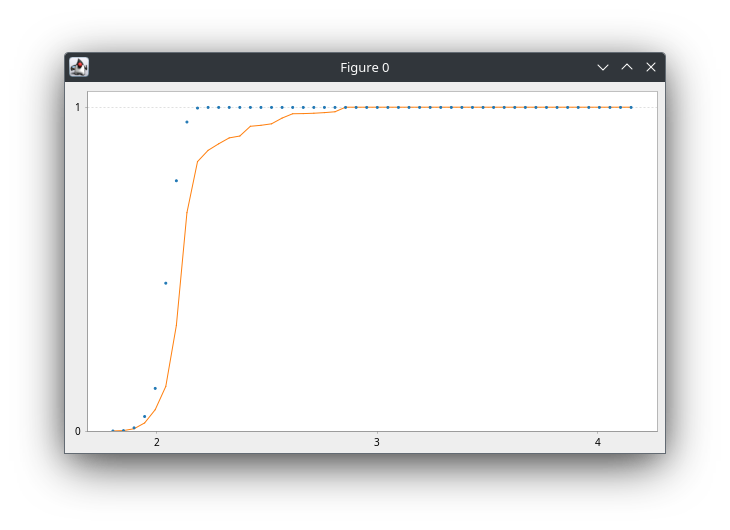
\includegraphics[scale=0.5]{images/lege11}
        \caption{Многочлены Лежандра, $X_0 = 1.1$}
    \end{figure}

    \newpage

    \begin{figure}[h]
        \centering
        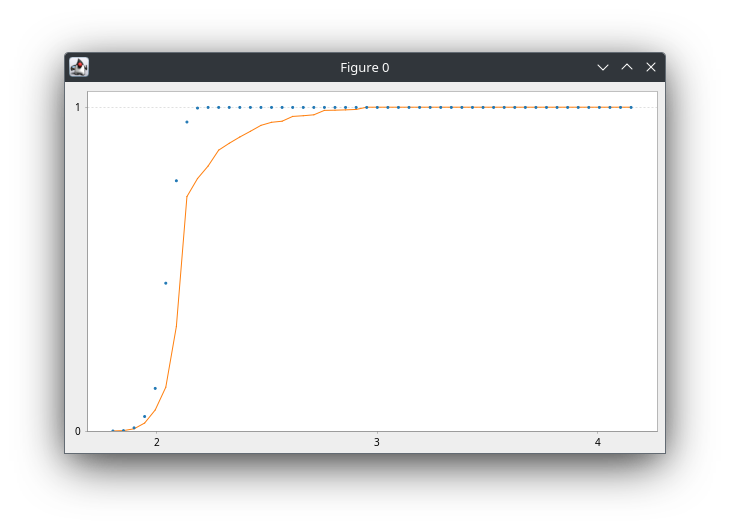
\includegraphics[scale=0.5]{images/poly11}
        \caption{Обыкновенные многочлены, $X_0 = 1.1$}
    \end{figure}

    \begin{figure}[h]
        \centering
        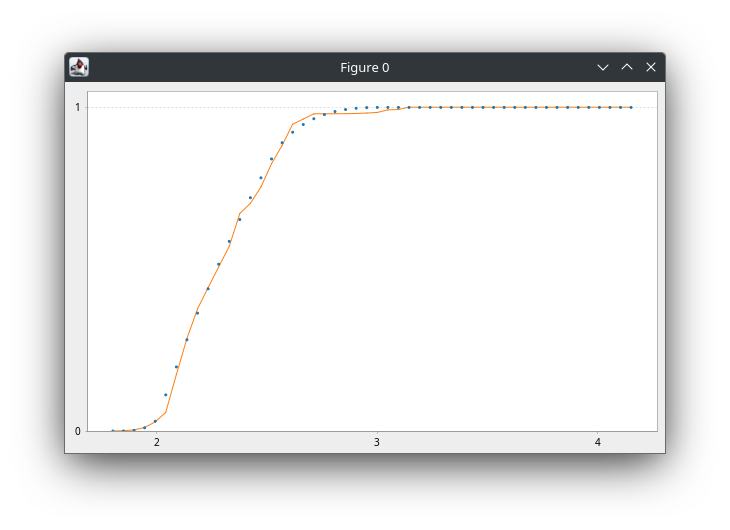
\includegraphics[scale=0.5]{images/lege15}
        \caption{Многочлены Лежандра, $X_0 = 1.5$}
    \end{figure}


    \begin{figure}[h]
        \centering
        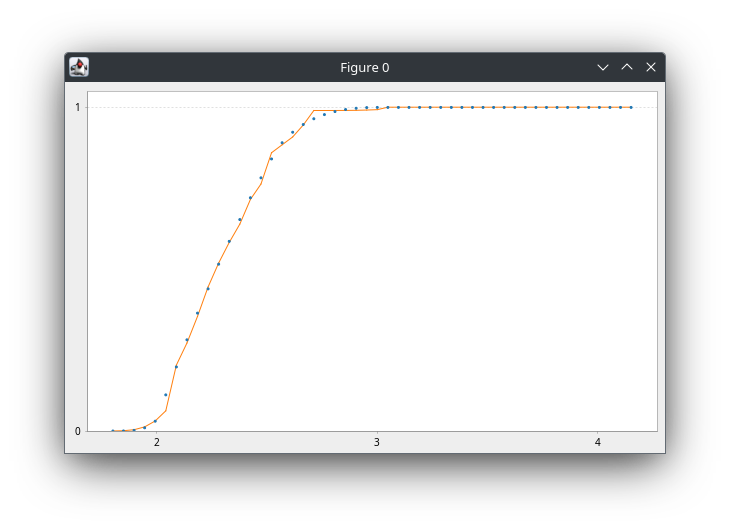
\includegraphics[scale=0.5]{images/poly15}
        \caption{Обыкновенные многочлены, $X_0 = 1.5$}
    \end{figure}

    \newpage

    \begin{figure}[h]
        \centering
        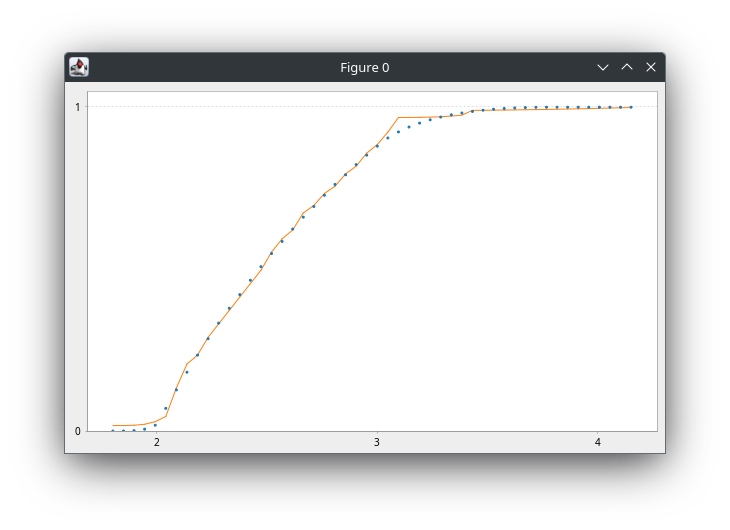
\includegraphics[scale=0.5]{images/lege19}
        \caption{Многочлены Лежандра, $X_0 = 1.9$}
    \end{figure}

    \newpage

    \begin{figure}[h]
        \centering
        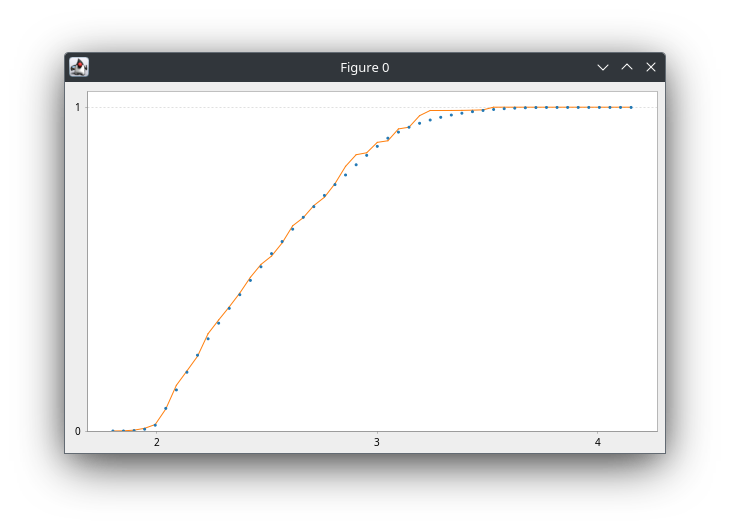
\includegraphics[scale=0.5]{images/poly19}
        \caption{Обыкновенные многочлены, $X_0 = 1.9$}
    \end{figure}
    \begin{figure}[h]
        \centering
        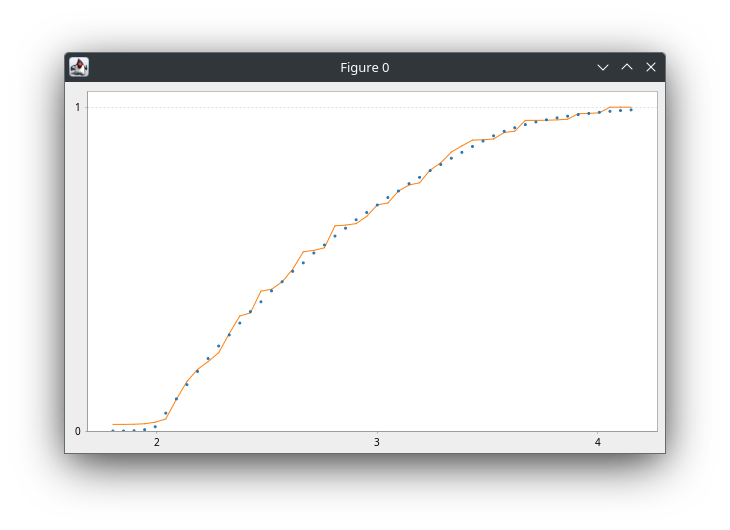
\includegraphics[scale=0.5]{images/lege23}
        \caption{Многочлены Лежандра, $X_0 = 2.3$}
    \end{figure}

    \newpage

    \begin{figure}[h]
        \centering
        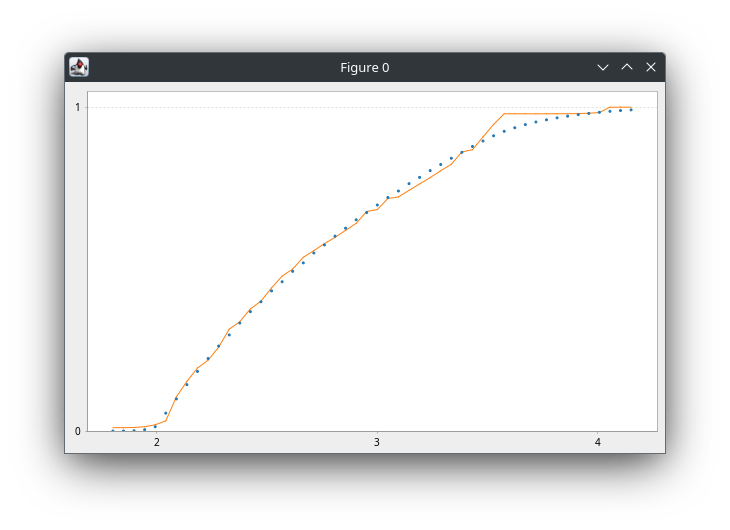
\includegraphics[scale=0.5]{images/poly23}
        \caption{Обыкновенные многочлены, $X_0 = 2.3$}
    \end{figure}
    \newpage

    \section*{Заключение}
    \addcontentsline{toc}{section}{Заключение}

    Был построен алгоритм, позволяющий при заданных
    параметрах системы частиц построить аппроксимацию
    для потенциала Гей-Берне, описывающего их взаимодействие.

    На данный момент вопрос скорости сходимости алгоритма
    и итоговой погрешности в зависимости от погрешностей
    всех использованных аппроксимаций, а также оптимального
    подбора регуляризационного параметра $\alpha$ остаётся
    открыт, однако использование при вычислении направления
    и длины шага в итерационном процессе аналитического
    выражения для производной позволяет выдвинуть гипотезу
    о квадратичной скорости сходимости метода, аналогично
    методу Ньютона.

    \newpage

    \section*{Список литературы}
    \addcontentsline{toc}{section}{Список литературы}

    \begingroup
    \renewcommand{\section}[2]{}% убираем автоматическую геренацию секции "список литературы"
    \begin{thebibliography}{99}

        \bibitem{bib:three}
        Sacanna, Stefano and Rossi, Laura and Pine, David J., Magnetic Click Colloidal Assembly. J. Am. Chem. Soc., 2012. 6112-6115 p.

        \bibitem{bib:four}
        Guangyu Liu and Longyu Li and Xinlin Yang, Preparation of ellipsoidal hematite/polymer hybrid materials and the corresponding hollow polymer ellipsoids. Polymer, 2008. 4776 - 4783 p

        \bibitem{bib:five}
        Nakade, Masato and Ikeda, Tetsuro and Ogawa, Makoto, Synthesis and properties of ellipsoidal hematite/silicone core-shell particles. Kluwer Academic Publishers-Plenum Publishers, 2007. 4815-4823 p.

        \bibitem{bib:six}
        M. Klinkigt and R. Weeber and S. Kantorovich and C. Holm, System of particles with shifted magnetic dipoles. Magnetohydrodynamics, 2011. 143-148 p.

        \bibitem{bib:seven}
        Arduengo, III, Anthony J. and H. V. Rasika Dias and Richard L. Harlow and Michael Kline, Electronic stabilization of nucleophilic carbenes. J. Am. Chem. Soc., 1992. 5530–5534 p

        \bibitem{bib:eight}
        Angel Abarca and Pilar Gomez-Sal and Avelino Martin and Miguel Mena and Josep Maria Poblet and Carlos Yelamos, Ammonolysis of mono(pentamethylcyclopentadienyl) titanium(iv) derivatives. Inorg. Chem., 2000. 642–651 p.

        \bibitem{bib:nine}
        ACoghill, Anne M. and Garson, Lorrin R., Ammonolysis of mono(pentamethylcyclopentadienyl) titanium(iv) derivatives. Oxford University Press, Inc. and The American Chemical Society

        \bibitem{bib:ten}
        Appelhans, Leah N. and Zuccaccia, Daniele and Kovacevic, Anes and Chianese, Anthony R. and Miecznikowski, John R. and Macchioni, Aleco and Clot, Eric and Eisenstein, Odile and Crabtree, Robert H., An aniondependent switch in selectivity results from a change of C-H activation mechanism in the reaction of an imidazolium salt with IrH5(PPh3)2. J. Am. Chem. Soc., 2005. 16299–16311 p.

        \bibitem{bib:one}
        Sofia Kantorovich, Elena Pyanzina, Cristiano De Michele and Francesco Sciortino, How to calculate structure factors of self-assembling anisotropic particles. Soft matter, 2013. 16 p.

        \bibitem{bib:two}
        Sofia Kantorovich, Elena Pyanzina and Francesco Sciortino, The influence of shape anisotropy on the microstructure of magnetic dipolar particles. Soft matter, 2010. 10 p.

        \bibitem{bib:Jonca:1988}
        Katarzyna Kuglarz Jonca: Numerical solution of a nonlinear Fredholm integral equation of the first kind. Montana State University (1988)

    \end{thebibliography}
    \endgroup

\end{document}